\documentclass{article}
\usepackage[utf8]{inputenc}
\usepackage{amsmath}
\usepackage{amssymb}
\usepackage{graphicx}

\begin{document}

% Aufgabe
\subsection*{Aufgabe}
Zeichne den Graphen der folgenden Funktionen, um ein Gespür für sie zu bekommen:
\begin{itemize}
  \item $\sin, \ \cos, \ \tan$
  \item $\sinh, \ \cosh, \ \tanh$
\end{itemize}

\subsection*{Lösung}

Um ein Gespür für die trigonometrischen und hyperbolischen Funktionen zu bekommen, zeichnen wir ihre Graphen und analysieren ihre wichtigsten Eigenschaften.

\subsubsection*{Trigonometrische Funktionen}

\textbf{1. Die Sinusfunktion $\sin(x)$}

Die Sinusfunktion ist eine periodische Funktion mit Periode $2\pi$. Sie nimmt Werte zwischen $-1$ und $1$ an.

\begin{figure}[!htbp]
\centering
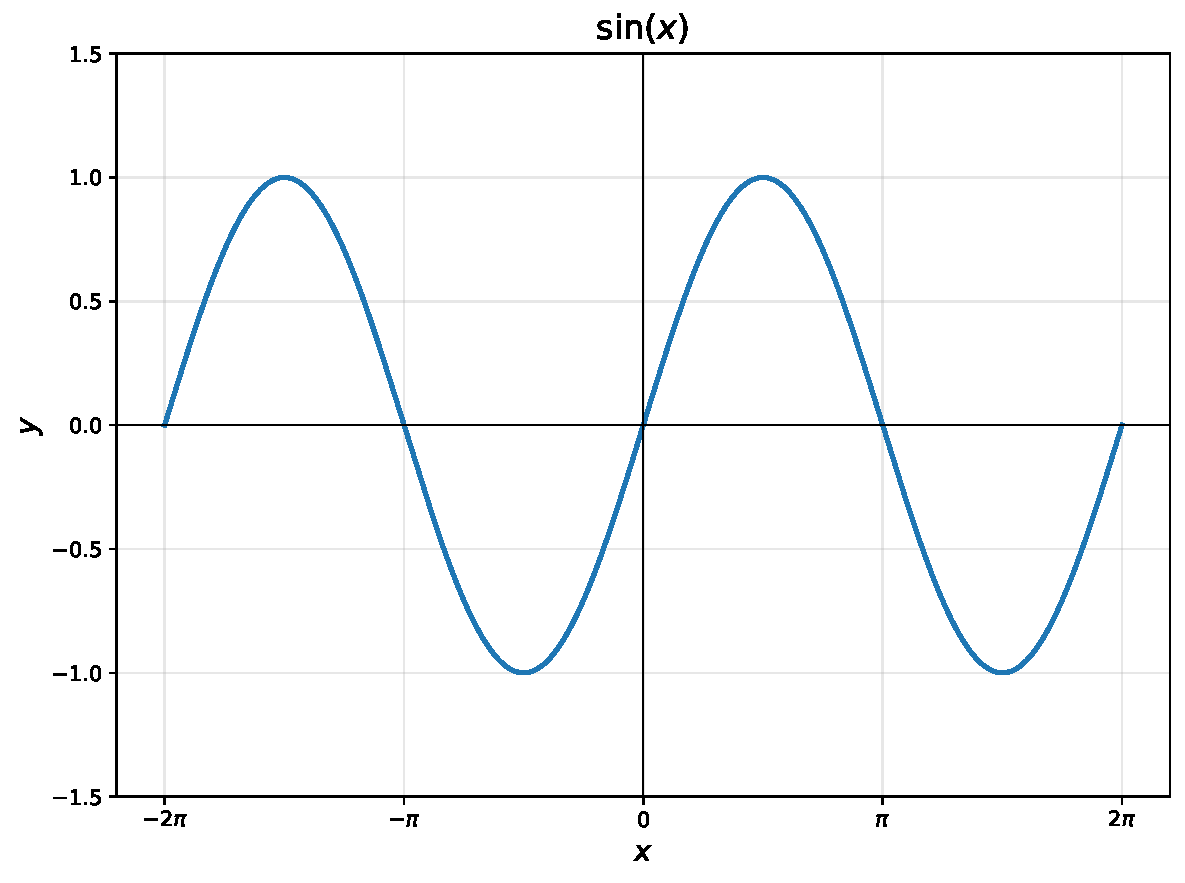
\includegraphics[width=0.8\textwidth]{sin.pdf}
\caption{Graph der Sinusfunktion}
\end{figure}

Wichtige Eigenschaften:
\begin{itemize}
\item Definitionsbereich: $\mathbb{R}$
\item Wertebereich: $[-1, 1]$
\item Periode: $2\pi$
\item Nullstellen: $x = k\pi$ für $k \in \mathbb{Z}$
\item Ungerade Funktion: $\sin(-x) = -\sin(x)$
\end{itemize}

\textbf{2. Die Kosinusfunktion $\cos(x)$}

Die Kosinusfunktion ist ebenfalls periodisch mit Periode $2\pi$ und nimmt Werte zwischen $-1$ und $1$ an.

\begin{figure}[!htbp]
\centering
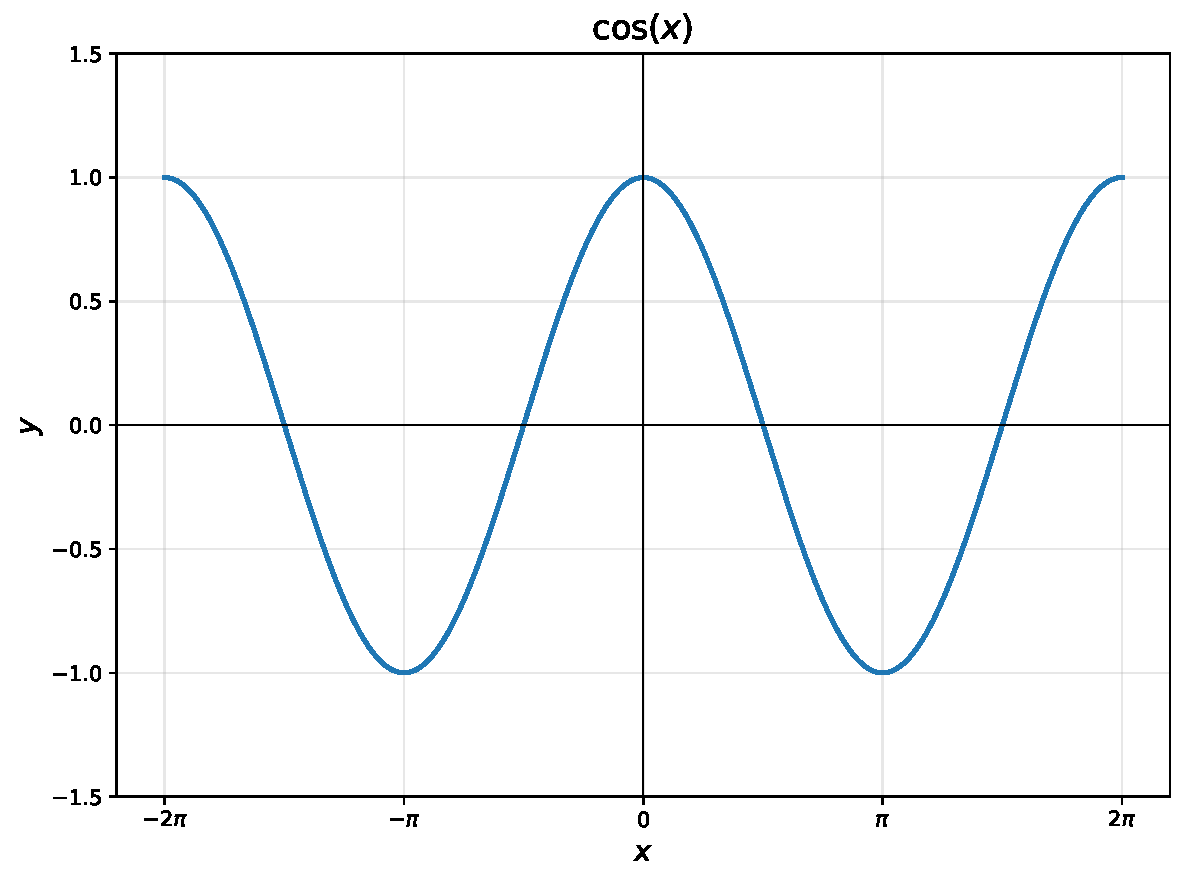
\includegraphics[width=0.8\textwidth]{cos.pdf}
\caption{Graph der Kosinusfunktion}
\end{figure}

Wichtige Eigenschaften:
\begin{itemize}
\item Definitionsbereich: $\mathbb{R}$
\item Wertebereich: $[-1, 1]$
\item Periode: $2\pi$
\item Nullstellen: $x = \frac{\pi}{2} + k\pi$ für $k \in \mathbb{Z}$
\item Gerade Funktion: $\cos(-x) = \cos(x)$
\item Beziehung zum Sinus: $\cos(x) = \sin(x + \frac{\pi}{2})$
\end{itemize}

\textbf{3. Die Tangensfunktion $\tan(x)$}

Die Tangensfunktion ist definiert als $\tan(x) = \frac{\sin(x)}{\cos(x)}$ und hat Polstellen an den Nullstellen des Kosinus.

\begin{figure}[!htbp]
\centering
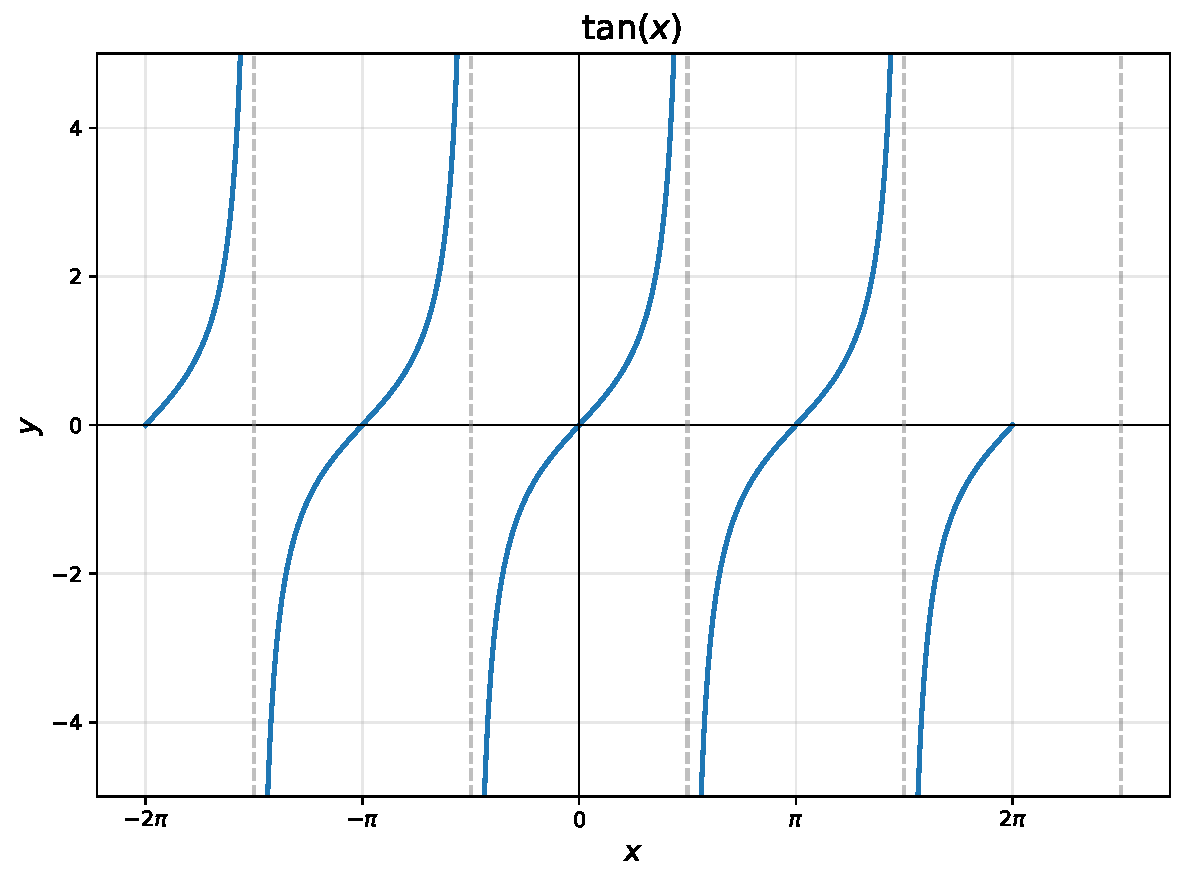
\includegraphics[width=0.8\textwidth]{tan.pdf}
\caption{Graph der Tangensfunktion}
\end{figure}

Wichtige Eigenschaften:
\begin{itemize}
\item Definitionsbereich: $\mathbb{R} \setminus \{\frac{\pi}{2} + k\pi : k \in \mathbb{Z}\}$
\item Wertebereich: $\mathbb{R}$
\item Periode: $\pi$
\item Nullstellen: $x = k\pi$ für $k \in \mathbb{Z}$
\item Polstellen (vertikale Asymptoten): $x = \frac{\pi}{2} + k\pi$ für $k \in \mathbb{Z}$
\item Ungerade Funktion: $\tan(-x) = -\tan(x)$
\end{itemize}

\subsubsection*{Hyperbolische Funktionen}

Die hyperbolischen Funktionen sind durch Exponentialfunktionen definiert und haben ähnliche Eigenschaften wie ihre trigonometrischen Gegenstücke, jedoch ohne Periodizität.

\textbf{4. Die hyperbolische Sinusfunktion $\sinh(x)$}

Der hyperbolische Sinus ist definiert als $\sinh(x) = \frac{e^x - e^{-x}}{2}$.

\begin{figure}[!htbp]
\centering
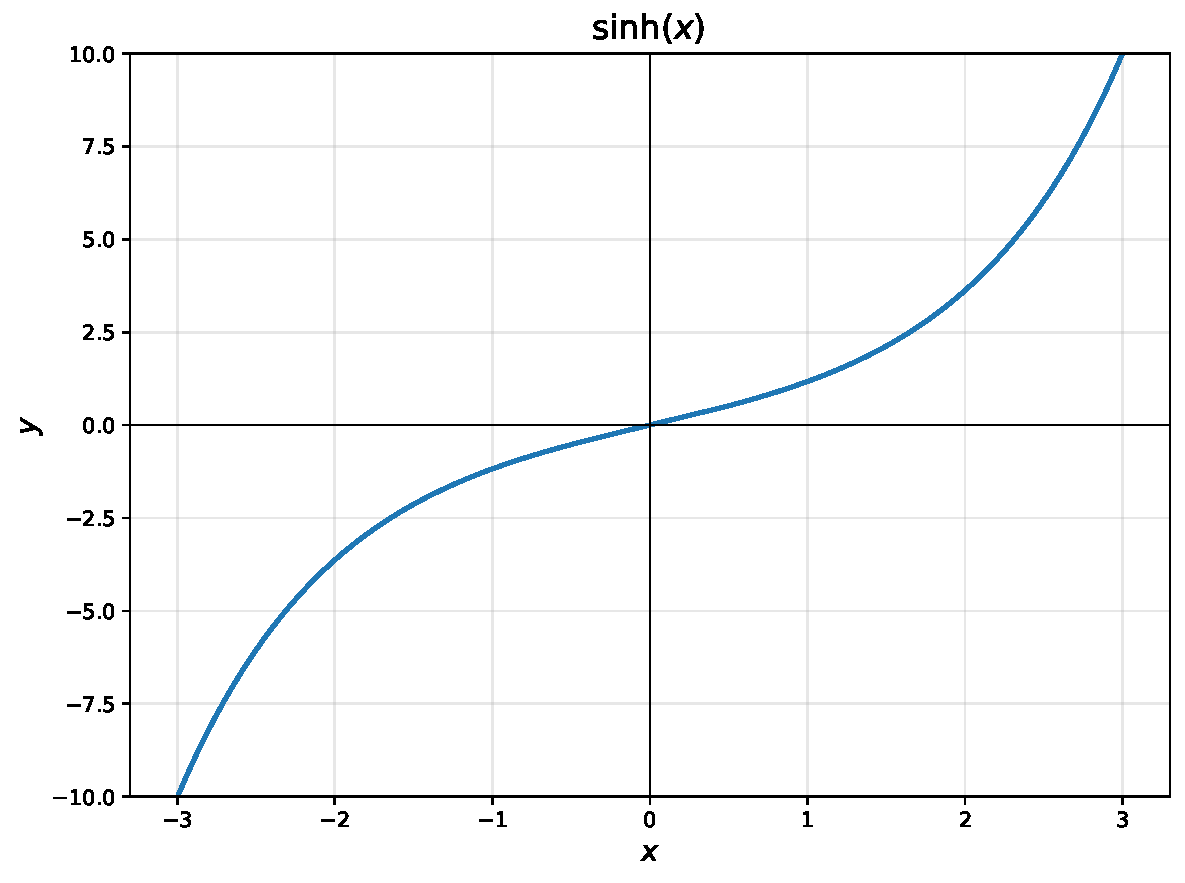
\includegraphics[width=0.8\textwidth]{sinh.pdf}
\caption{Graph der hyperbolischen Sinusfunktion}
\end{figure}

Wichtige Eigenschaften:
\begin{itemize}
\item Definitionsbereich: $\mathbb{R}$
\item Wertebereich: $\mathbb{R}$
\item Keine Periode
\item Einzige Nullstelle: $x = 0$
\item Ungerade Funktion: $\sinh(-x) = -\sinh(x)$
\item Asymptotisches Verhalten: $\sinh(x) \approx \frac{e^x}{2}$ für $x \to \infty$ und $\sinh(x) \approx -\frac{e^{-x}}{2}$ für $x \to -\infty$
\end{itemize}

\textbf{5. Die hyperbolische Kosinusfunktion $\cosh(x)$}

Der hyperbolische Kosinus ist definiert als $\cosh(x) = \frac{e^x + e^{-x}}{2}$.

\begin{figure}[!htbp]
\centering
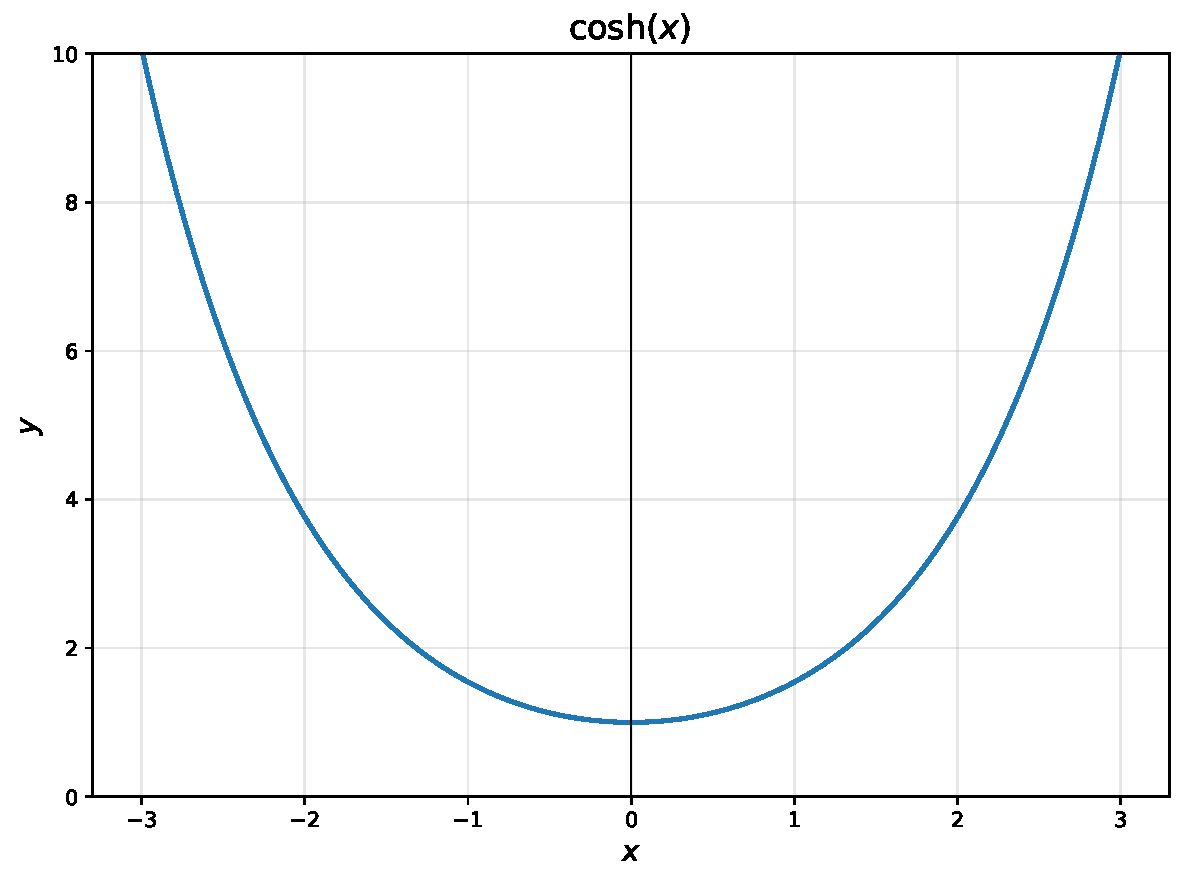
\includegraphics[width=0.8\textwidth]{cosh.pdf}
\caption{Graph der hyperbolischen Kosinusfunktion}
\end{figure}

Wichtige Eigenschaften:
\begin{itemize}
\item Definitionsbereich: $\mathbb{R}$
\item Wertebereich: $[1, \infty)$
\item Keine Periode
\item Keine Nullstellen
\item Gerade Funktion: $\cosh(-x) = \cosh(x)$
\item Minimum bei $x = 0$ mit $\cosh(0) = 1$
\item Asymptotisches Verhalten: $\cosh(x) \approx \frac{e^{|x|}}{2}$ für $|x| \to \infty$
\end{itemize}

\textbf{6. Die hyperbolische Tangensfunktion $\tanh(x)$}

Der hyperbolische Tangens ist definiert als $\tanh(x) = \frac{\sinh(x)}{\cosh(x)} = \frac{e^x - e^{-x}}{e^x + e^{-x}}$.

\begin{figure}[!htbp]
\centering
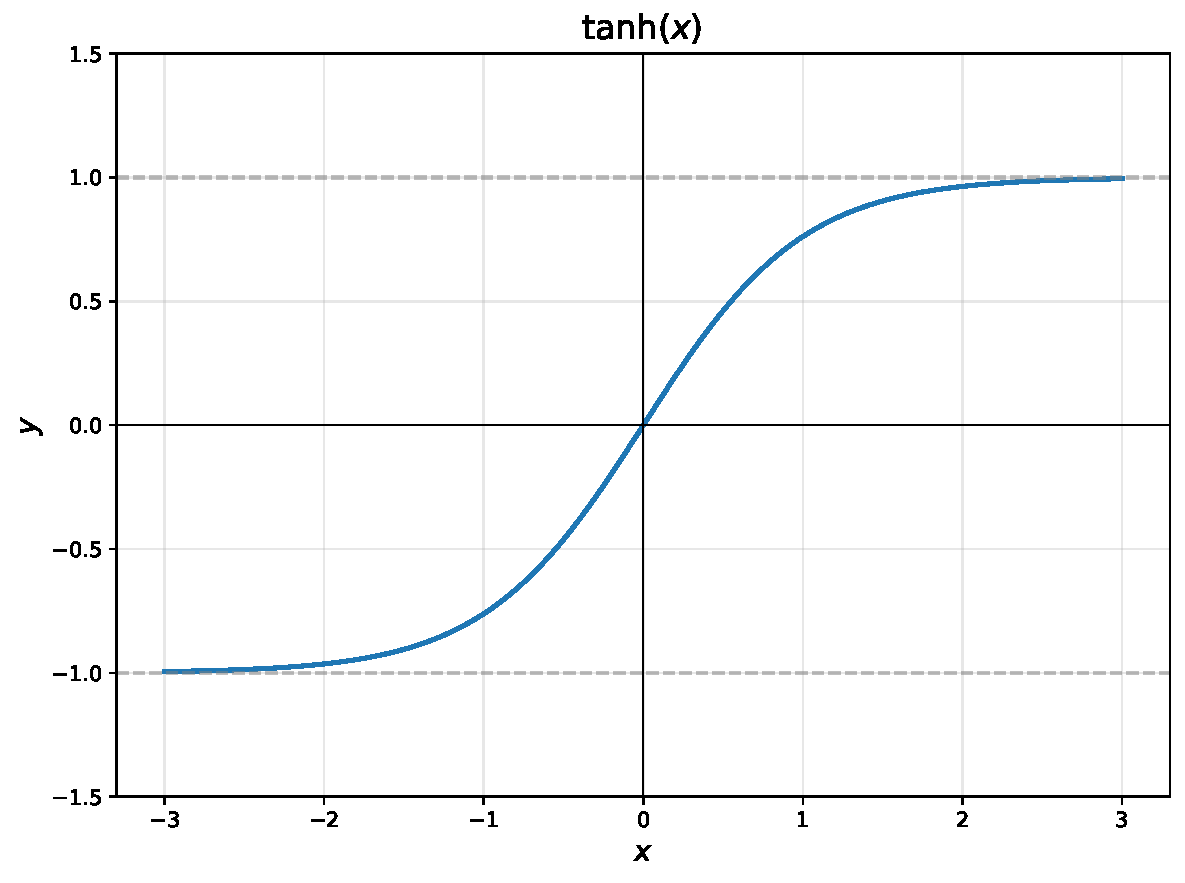
\includegraphics[width=0.8\textwidth]{tanh.pdf}
\caption{Graph der hyperbolischen Tangensfunktion}
\end{figure}

Wichtige Eigenschaften:
\begin{itemize}
\item Definitionsbereich: $\mathbb{R}$
\item Wertebereich: $(-1, 1)$
\item Keine Periode
\item Einzige Nullstelle: $x = 0$
\item Ungerade Funktion: $\tanh(-x) = -\tanh(x)$
\item Horizontale Asymptoten: $y = 1$ für $x \to \infty$ und $y = -1$ für $x \to -\infty$
\item Streng monoton wachsend
\end{itemize}

\subsubsection*{Vergleich und Zusammenfassung}

\begin{figure}[!htbp]
\centering
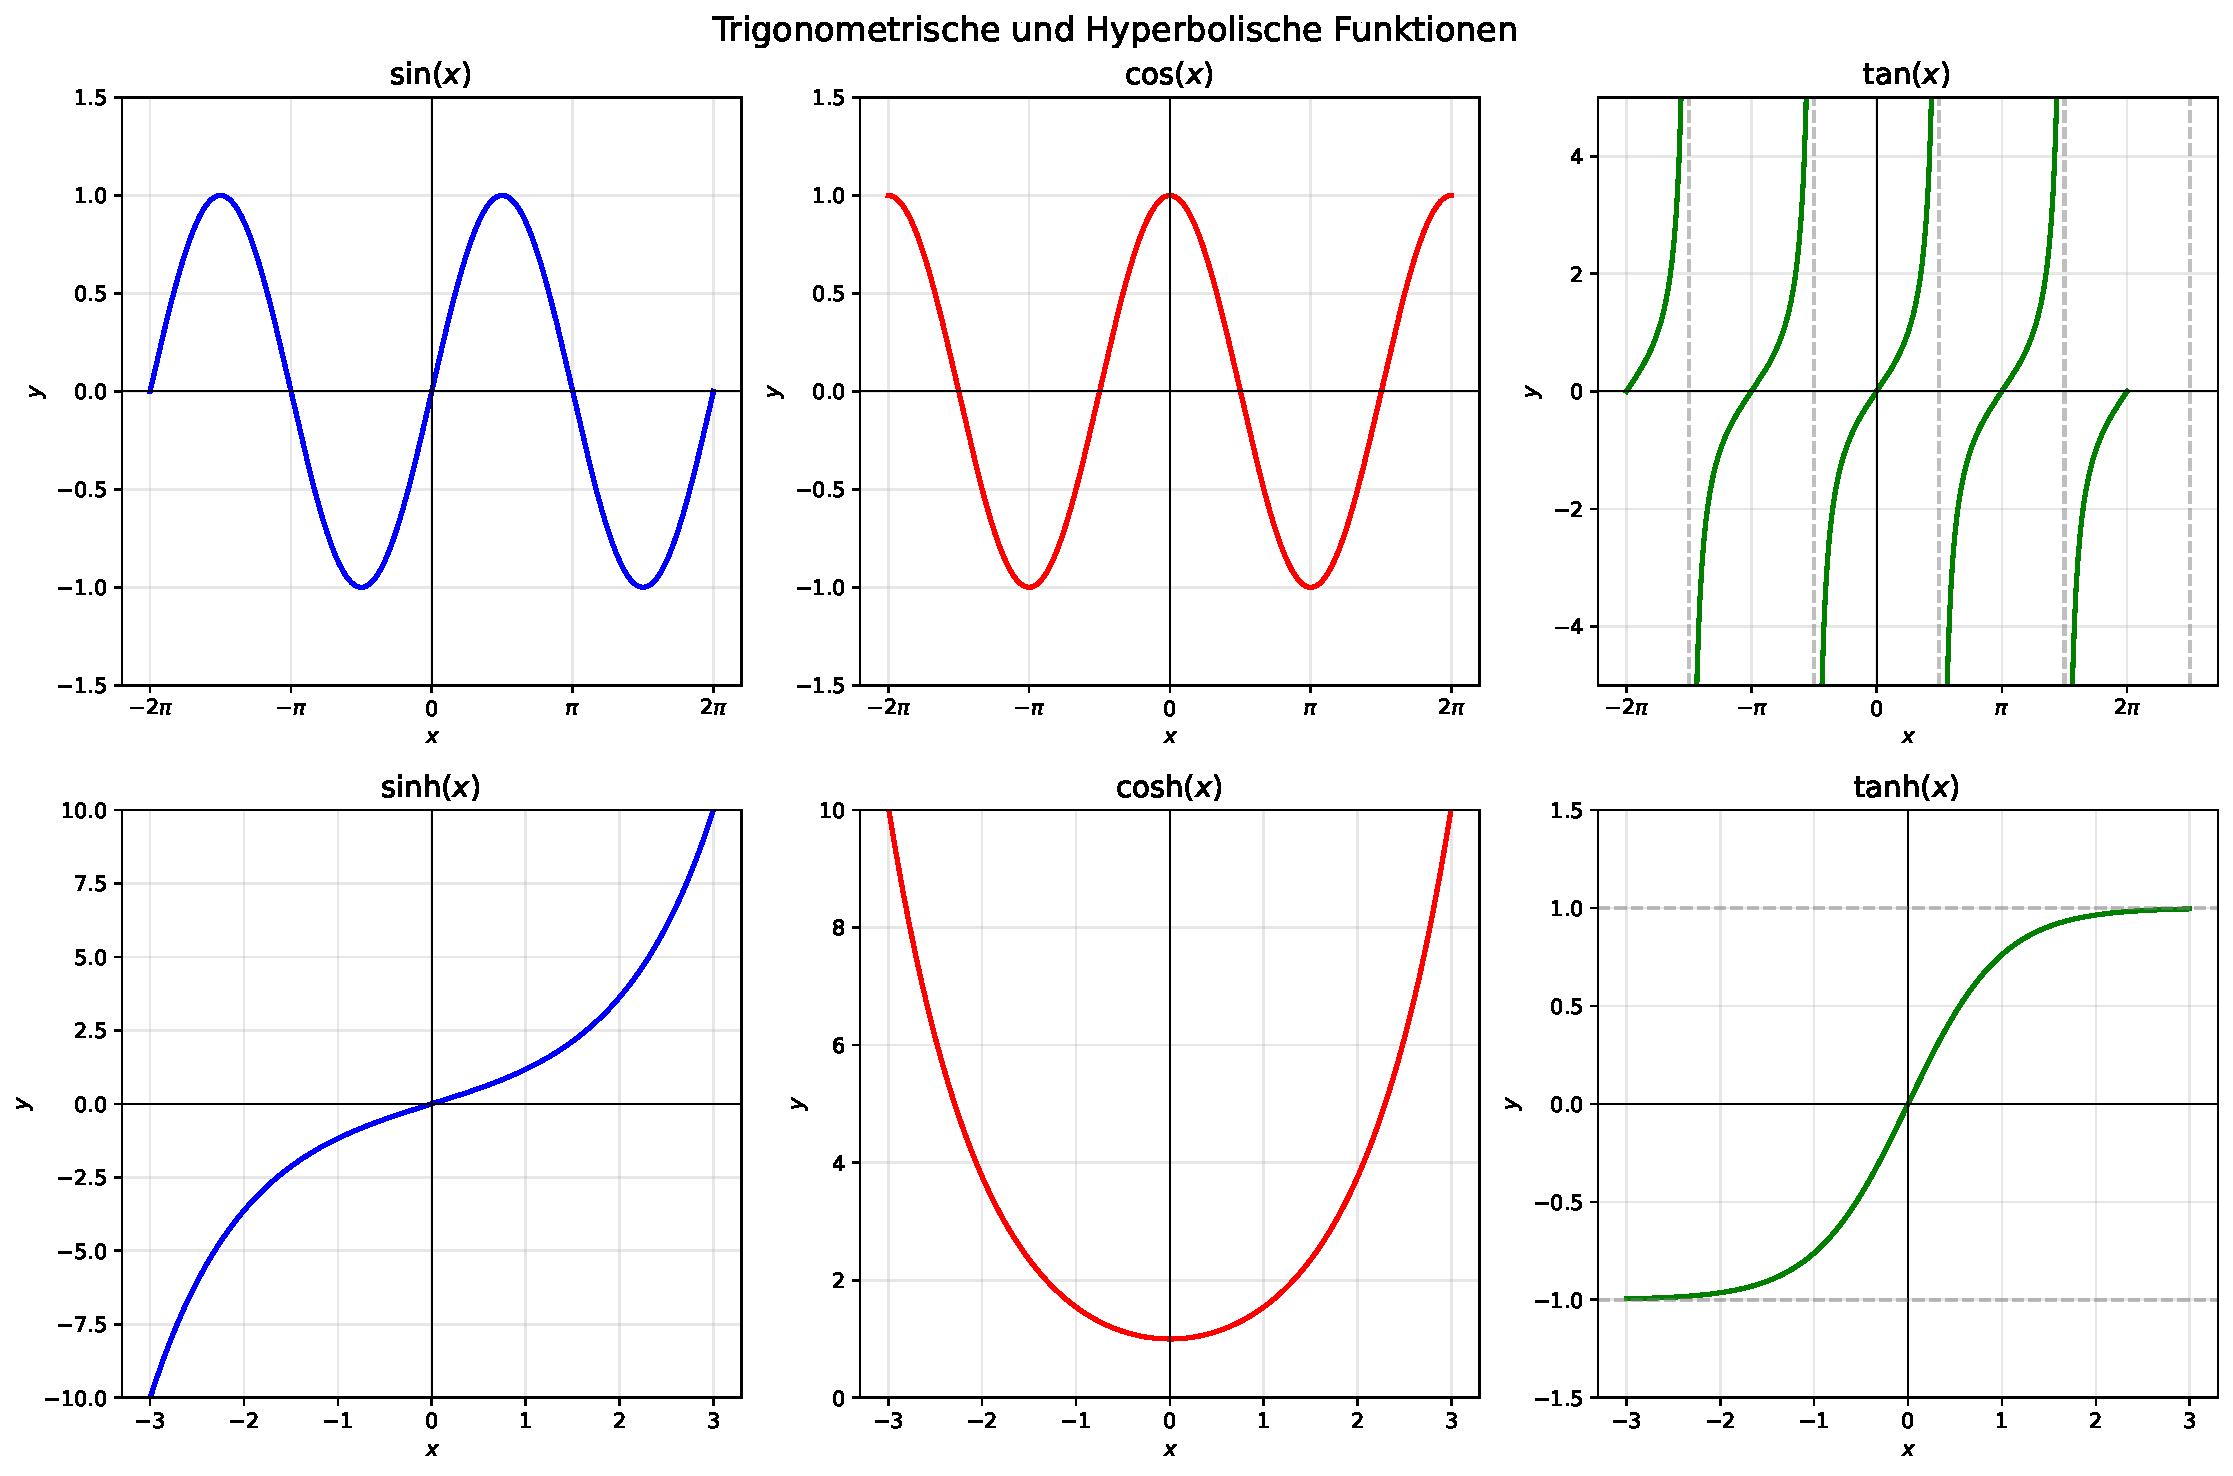
\includegraphics[width=\textwidth]{function_graphs.pdf}
\caption{Übersicht aller sechs Funktionen}
\end{figure}

Die trigonometrischen und hyperbolischen Funktionen zeigen sowohl Ähnlichkeiten als auch wichtige Unterschiede:

\textbf{Ähnlichkeiten:}
\begin{itemize}
\item Sinus und hyperbolischer Sinus sind beide ungerade Funktionen
\item Kosinus und hyperbolischer Kosinus sind beide gerade Funktionen
\item Tangens und hyperbolischer Tangens sind beide ungerade Funktionen
\item Es gelten ähnliche Identitäten, z.B. $\sin^2(x) + \cos^2(x) = 1$ und $\cosh^2(x) - \sinh^2(x) = 1$
\end{itemize}

\textbf{Unterschiede:}
\begin{itemize}
\item Trigonometrische Funktionen sind periodisch, hyperbolische nicht
\item Trigonometrische Funktionen sind beschränkt (außer $\tan$), hyperbolische wachsen exponentiell (außer $\tanh$)
\item Die Nullstellen und Extremstellen unterscheiden sich grundlegend
\end{itemize}

Diese Funktionen spielen eine zentrale Rolle in vielen Bereichen der Mathematik und Physik, von der Beschreibung von Schwingungen (trigonometrische Funktionen) bis zur Relativitätstheorie (hyperbolische Funktionen).

\end{document}